\documentclass{article}

\title{Finding Optimal Solutions for Alternative Feature Selection}
\author{Jakob Bach}

\usepackage[style=ieee, backend=bibtex]{biblatex}
\usepackage[ruled,linesnumbered,vlined]{algorithm2e} % pseudo-code
\usepackage{amsmath} % mathematical symbols
\usepackage{amssymb} % mathematical symbols
\usepackage{amsthm} % theorems, definitions etc.
\usepackage{graphicx} % plots
\usepackage{subcaption} % figures with multiple sub-figures and sub-captions
\usepackage{hyperref} % links and URLs
\addbibresource{references.bib}

\theoremstyle{definition}
\newtheorem{definition}{Definition}

\begin{document}

\maketitle

\begin{abstract}
Feature-selection methods are popular to obtain small, interpretable, yet highly accurate prediction models.
Existing feature-selection methods typically yield either a fixed set of features or a ranking of features.
However, obtaining just one feature set might not be sufficient in some cases.
For example, users might be interested in finding different feature sets with similar prediction quality, offering alternative explanations of the data.
In this article, we formalize alternative feature selection as optimization problem.
Next, we propose several general approaches to solve this problem.
In particular, we show how to integrate various kinds of existing feature-selection methods.
Finally, we evaluate these approaches in a study with classification datasets.
In our experiments, we find that most datasets give way to finding alternative feature sets with similar prediction quality as the optimal ones.
\end{abstract}

\textbf{Keywords:} feature selection, alternatives, constraints, explainability

\section{Introduction}
\label{sec:introduction}

\paragraph{Motivation}

Feature-selection methods are ubiquitous for a variety of reasons.
By reducing the dimensionality of the dataset, they lower computational and memory requirements of prediction models.
Next, models might generalize better if irrelevant and spurious predictors are removed.
Finally, prediction models might be smaller and more comprehensive due to feature selection~\cite{li2017feature}, improving interpretability.

Traditional feature-selection methods either select a feature set or assign a score to each feature.
One can derive a feature set from the latter by only selecting the top-ranked features.
In any case, existing methods focus on optimizing a criterion of feature-set quality, e.g., prediction performance.
However, besides the optimal feature set, there might be multiple, differently composed feature sets with similar quality.
For the user, these other feature sets might be interesting alternatives for multiple reasons.
First, some of the originally selected features might be costly to obtain, so the user would prefer cheaper alternatives, while maintaining prediction quality.
Second, some of the originally selected features might contain sensitive information that should not be used in predictions.
Third, the user might be interested in explaining the prediction target, rather than just making good predictions.
In such a situation, knowing alternatives allows for formulating multiple hypotheses and broadens the understanding.

\paragraph{Problem statement}

This article addresses the problem of alternative feature selection, which we informally define as follows:
%
\begin{definition}[Alternative feature selection (informal)]
	Given an original feature set, find a sufficiently different feature set that optimizes feature-set quality at the same time.
	\label{def:alternative-feature-selection}
\end{definition}
%
We provide formal definitions later.
If the original feature set had high quality, the alternative feature set should have a similar quality.
Depending on how different the alternative feature set should be, one might have to compromise on quality.
E.g., if there are only a few highly predictive features and most of them are part of the original feature set, the alternative feature set might have significantly lower prediction quality.
We analyze this effect in our article.
Also, we consider finding multiple alternatives rather than just one.

Two points are essential for alternative feature selection, which we both address in this article.
First, one needs to formalize and quantify what an alternative feature sets is.
Second, one needs an approach to efficiently find alternative feature sets.
Ideally, the approach should be general, i.e., cover a broad range of existing feature-selection methods.

\paragraph{Related work}

In machine learning, finding alternative solutions has already been addressed extensively in clustering~\cite{bae2006coala}.
However, there is a lack of such approaches and corresponding experimental evaluation for feature selection.
The concept of statistically equivalent feature subsets~\cite{lagani2017feature} groups features such that one obtains alternatives for each individual feature.
However, there might not be such an alternative for some features.
Also, we consider alternatives to feature sets as a whole.
In the field of explainable AI, counterfactual explanations have massively gained popularity in the last few years~\cite{verma2020counterfactual, stepin2021survey}.
Such explanations involve data objects with similar feature values, but a different prediction.
In contrast, we target at different feature sets with similar feature-set quality, e.g., prediction performance.

\paragraph{Contributions}

Our contribution is threefold.
First, we define an optimization problem that formalizes alternative feature selection.
We foster the search for alternatives via constraints on feature sets.
This formulation also allows integrating other constraint types on feature sets~\cite{paclik2002feature,yuan2006model,groves2015toward}.
Second, we propose heuristic and exact approaches to solve this optimization problem.
To that end, we discuss how to integrate different kinds of feature-selection methods in the objective function.
Our notion of alternative feature sets is general and thus not tailored towards specific feature-selection methods.
Third, we evaluate our approaches for alternative feature selection with comprehensive experiments.
We use 30 classification dataset from the Penn Machine Learning Benchmarks (PMLB)~\cite{olson2017pmlb, romano2021pmlb} and four different feature-selection methods.
We focus on the question if one can find alternative feature sets with similar feature-set quality as the original ones.

\paragraph{Results}

We find that most datasets allow finding alternative feature sets with similar quality as the optimal ones.
This presents the user with alternative explanations for high-quality predictions.
For the different feature-selection methods, we note \dots
Comparing search configurations for alternatives, we find \dots
We publish our code\footnote{\url{https://github.com/Jakob-Bach/AFS}} and our experimental data\footnote{temporary link: \url{https://bwsyncandshare.kit.edu/s/xxx}; will be moved to a public repository after review}.

\paragraph{Outline}

Section~\ref{sec:fundamentals} explains fundamentals of feature selection.
Section~\ref{sec:approach} defines the optimization problem of alternative feature selection and discusses approaches to solve it.
Section~\ref{sec:related-work} reviews related work.
Section~\ref{sec:experimental-design} describes our experimental design.
Section~\ref{sec:evaluation} presents the experimental results.
Section~\ref{sec:conclusion} concludes.

\section{Fundamentals}
\label{sec:fundamentals}

In this section, we introduce basic notation and review different methods to measure quality of feature sets.

\subsection{Notation}
\label{sec:fundamentals:notation}

Let $X \in \mathbb{R}^{m \times n}$ be a dataset represented as a matrix.
Each row is a data object, and each column is a feature.
Let $F = \{f_1, \dots, f_n\}$ denote the set of feature names.
We assume categorical features have already been made numeric, e.g., via one-hot encoding.
Let $X_{\cdot{}j} \in \mathbb{R}^m$ denote the vector representation of the $j$-th feature.
Further, let $y \in \mathbb{R}^m$ represent the prediction target.
The actual domain of the target might also be smaller, e.g., $\{0,1\}$ for binary classification.

With feature selection, one makes a binary decision $s_j \in \{0,1\}$ for each feature, i.e., either selects it or not.
The vector $s \in \{0,1\}^n$ combines all these selection decisions.
The selected feature set is $F_s = \{f_j \mid s_j=1\}$.
Let the function $Q(s,X,y)$ return the quality of a such feature set.
Without loss of generality, we assume this function should be maximized.

\subsection{Measuring Feature (Set) Quality}
\label{sec:fundamentals:quality}

There are different ways to evaluate feature-set quality $Q(s,X,y)$.
Note that we only give a short overview here, and focus on methods that we use in our evaluation.
See \cite{chandrashekar2014survey,li2017feature} for comprehensive surveys of feature selection.
A typical categorization of feature selection is into filter, wrapper, and embedded methods~\cite{guyon2003introduction}.

\paragraph{Filter methods}

Filter methods evaluate feature sets without training a prediction model.
Univariate filters assess each feature on its own, often assigning a numeric score ot each feature, while multivariate filters evaluate feature sets.
Examples for univariate filters are the absolute Pearson correlation or the mutual information between a feature and the prediction target.
Such methods ignore potential interaction between features, e.g., if they are redundant to each other.
Multivariate methods often combine a measure of feature relevance with a measure of feature redundancy.
Examples for such a method include CFS \cite{hall1999correlation}, FCBF \cite{yu2003feature}, and mRMR \cite{peng2005feature}.
Another interesting filter method is Relief~\cite{kira1992feature}, for which multiple extensions exist.
While Relief assigns quality to individual features rather than feature sets, it still uses other features indirectly via nearest-neighbor computations between data objects.

\paragraph{Wrapper methods}

Wrapper methods~\cite{kohavi1997wrappers} employ a search strategy over feature sets and evaluate each of these feature set by training a prediction model.
Thus, feature-set quality is equal to the prediction quality of the model trained with this feature set.
Various black-box optimization techniques can serve as search strategy, e.g., genetic algorithms.

\paragraph{Embedded methods}

Embedded methods train prediction models with built-in feature selection, e.g., decision trees~\cite{breiman1984classification} or random forests~\cite{breiman2001random}.
Thus, the criterion to evaluate the quality of features or feature sets is model-specific.
For example, tree-based models often use information gain or the Gini index to select features during training.

\paragraph{Post-hoc feature-importance methods}

Apart from traditional feature selection, there are various methods that assess feature importance after training a model.
These methods range range from local explanation methods like LIME~\cite{ribeiro2016should} or SHAP~\cite{lundberg2017unified} to global importance methods like permutation importance~\cite{breiman2001random} or SAGE~\cite{covert2020understanding}.
In particular, assessing feature importance plays a crucial role in the emerging fields of ML interpretability~\cite{carvalho2019machine}.

\section{Alternative Feature Selection}
\label{sec:approach}

In this section, we present the problem and approaches for alternative feature selection.
First, we define the structure of the optimization problem, i.e., objective and constraints.
Second, we formalize the notion of alternatives via constraints.
Third, we discuss different objective functions, corresponding to different feature-set quality measures from Section~\ref{sec:fundamentals:quality}
In particular, we describe how to solve the resulting the optimization problem.

\subsection{Optimization Problem}
\label{sec:approach:problem}

In alternative feature selection, there are two goals.
First, the quality of an alternative feature set should be high.
Second, an alternative feature set should be different to one or more existing feature set(s).
There are different ways to combine these two goals in an optimization problem:

First, one can consider both goals as objectives, obtaining an unconstrained multi-objective problem.
Second, one can treat feature-set quality as objective and being alternative as one or multiple constraints.
Third, one can consider being alternative as objective and introduce a constraint on feature-set quality, e.g., a lower bound.
Fourth, one can define constraints for both feature-set quality and being alternative, searching for any feasible solution instead of optimizing.
Depending on the use case, any of these four formulations might be appropriate.

In accordance with the informal Definition~\ref{def:alternative-feature-selection} from the introduction, we stick to the second formulation, i.e., optimizing feature-set quality subject to being alternative.
This option has the advantage of keeping the original objective function of feature selection.
Consequently, one does not need to specify a range or a threshold on feature-set quality.
Instead, the user can control how alternative the feature set should be.
This yields the following optimization problem:
%
\begin{align}
	\max_s &\quad Q(s,X,y) \nonumber \\
	\text{subject to:} &\quad F_s~\text{being alternative}
\end{align}
%
We discuss different constraints for \emph{being alternative} and different objective functions $Q(s,X,y)$ in the following.

\subsection{Constraints -- Defining Alternative Feature Sets}
\label{sec:approach:constraints}

In this section, we formalize alternative feature sets.
First, we discuss the base case where an individual feature set is an alternative to another one.
Second, we extend this notion to multiple alternatives, considering sequential as well as simultaneous search procedures for alternatives.
Note that this part our work is independent from the feature-selection method one wants to use.

\subsubsection{Single Alternatives}
\label{sec:approach:constraints:single}

We consider a feature set to be an alternative to another feature set if it differs sufficiently.
Mathematically, we express this with a set-dissimilarity measure~\cite{egghe2009new}.
Most of these measures consider how strongly two sets overlap and set this in relation to the size of the sets.
For example, a simple and well-known set-dissimilarity measure is the Jaccard distance.
Given two feature sets $F_1$, $F_2$, the Jaccard distance is defined as
%
\begin{equation}
	d_{Jacc}(F_1,F_2) = 1 - \frac{|F_1 \cap F_2|}{|F_1 \cup F_2|} = 1 - \frac{|F_1 \cap F_2|}{|F_1| + |F_2| - |F_1 \cap F_2|}
	\label{eq:jaccard}
\end{equation}
%
We leverage such a dissimilarity measure for the following definition:
%
\begin{definition}[Pairwise alternative]
	A feature set $F_2$ is an alternative to a feature set $F_1$ (and vice versa) for a dissimilarity threshold $\tau \in [0,1]$ if $d(F_1,F_2) \geq \tau$.
	\label{def:single-alternative}
\end{definition}
%
Depending on the preferences of the user, different values of $\tau$ might be appropriate.
The choice of $\tau$ depends on how alternative the new feature set should be.
Also, a feature set that differs strongly might yield a large change in feature-set quality.
Thus, we leave $\tau$ as a parameter of our approach.
If the choice of $\tau$ is unclear a priori, users can try out different values and compare results.
If the set-dissimilarity measure is normalized to $[0,1]$, the interpretation of $tau$ is user-friendly:
A value of $0$ allows the alternative feature set to be identical to the original feature set.
A value of $1$ requires the two feature sets to have no overlap.

If the feature sets sizes $|F_1|$ and $|F_2|$ are known, a threshold $\tau$ corresponds to a particular maximum number of overlapping features $|F_1 \cap F_2|$.
This follows from re-arranging Equation~\ref{eq:jaccard} and adapting Definition~\ref{def:single-alternative} accordingly:
%
\begin{align}
	& & d_{Jacc}(F_1,F_2) = 1 - \frac{|F_1 \cap F_2|}{|F_1| + |F_2| - |F_1 \cap F_2|} &\geq \tau \nonumber \\
	&\Leftrightarrow & |F_1 \cap F_2| &\leq \frac{1 - \tau}{2 - \tau} \cdot (|F_1| + |F_2|)
	\label{eq:jaccard-rearranged}
\end{align}
%
The latter formulation avoids having the feature-set sizes, and thereby the decision variables, in a quotient.
However, we can see that the effect of setting $\tau$ on the overlap size is non-linear.
Thus, we resort to another set overlap measure in this article, the using Dice coefficient:
%
\begin{align}
	& & d_{Dice}(F_1,F_2) = 1 - \frac{2 \cdot |F_1 \cap F_2|}{|F_1| + |F_2|} &\geq \tau \nonumber \\
	&\Leftrightarrow & |F_1 \cap F_2| &\leq \frac{1 - \tau}{2} \cdot (|F_1| + |F_2|)
	\label{eq:dice-rearranged}
\end{align}
%
If $|F_1| = |F_2|$, this measure is also identical to several further overlap measures.
In that case, $\tau$ directly controls which fraction of features in one set needs to differ in the other set, and vice versa:
%
\begin{align}
	& &\text{If}~|F_1| = |F_2|: \quad d_{Dice}(F_1,F_2) &\geq \tau \nonumber \\
	&\Leftrightarrow & |F_1 \cap F_2| &\leq (1 - \tau) \cdot |F_1| = (1 - \tau) \cdot |F_2|
\end{align}
%
Up to now, we have worked with feature set sizes instead of the binary feature-selection vector $s$.
However, expressing the feature-set sizes in terms of $s$ is straightforward:
%
\begin{align}
	|F_s| =& \sum_{j=1}^n s_j \nonumber \\
	|F_{s_1} \cap F_{s_2}| =& \sum_{j=1}^n s_{1,j} \cdot s_{2,j}
	\label{eq:feature-set-size}
\end{align}
%
Combining Equation~\ref{eq:jaccard-rearranged} or Equation~\ref{eq:dice-rearranged} with Equation~\ref{eq:feature-set-size} yields an inequality only involving sums and products of the binary decision variables and constant values.
In fact, one can replace the product $s_{1,j} \cdot s_{2,j}$ with linear constraints by introducing an auxiliary variable $t_j$~\cite{mosek2021modeling}:
%
\begin{align}
	t_j \leq& s_{1,j} \nonumber \\
	t_j \leq& s_{2,j} \nonumber \\
	1 + t_j \geq& s_{1,j} + s_{2,j} \nonumber \\
	t_j \in& \{0,1\}
	\label{eq:product-linear}
\end{align}
%
Thus, one can express alternative features sets according to Definition~\ref{def:single-alternative} with 0-1 integer linear constraints.
This simple constraint type allows for using a broad range of solvers, given the right objective function, which we discuss in Section~\ref{sec:approach:objectives}.
If there is an existing feature set, i.e., one either knows $s_1$ or $s_2$, Equation~\ref{eq:feature-set-size} already is linear without applying Equation~\ref{eq:product-linear}.

\subsubsection{Multiple Alternatives}
\label{sec:approach:constraints:multiple}

If the user desires multiple alternative feature sets rather than just one, one can compute these alternatives either sequentially or simultaneously.

\paragraph{Sequential alternatives}

In the sequential case, the user gets several alternatives iteratively.
In each iteration, we determine one alternative feature set.
We constrain the new feature set to be alternative to all previously found feature sets:
%
\begin{definition}[Sequential alternative]
	A feature set $F_2$ an alternative to a set of feature sets $\mathbb{F}$ (and vice versa) for a dissimilarity threshold $\tau \in [0,1]$ if $\forall F_1 \in \mathbb{F}: d(F_1,F_2) \geq \tau$.
	\label{def:sequential-alternative}
\end{definition}
%
This definition effectively just duplicates the constraint from the base case and instantiates it for different existing feature sets.
The objective function remains the same as in the base case, i.e., we optimize the quality of the new feature set~$F_2$.
This means the number of variables in the optimization problem remains constant, independent from the number of alternatives.
Each alternative only adds one new constraint to the optimization problem.
As we are alway comparing a new, variable feature set to existing feature sets, we also do not need to introduce interaction variables as in Equation~\ref{eq:product-linear}.
Thus, we expect the runtime of sequential search to scale well with the number of alternatives.

As the solution space becomes narrower over iterations, feature-set quality can drop with each further alternative.
The user can decide after each iteration if feature-set quality is too low or if another alternative should be found.
Also, a solver for this problem might benefit runtime-wise from iteratively adding constraints, provided the solver keeps some internal state between iterations and can warm-start.

Instead of Definition~\ref{def:sequential-alternative}, one could also use a less strict constraint, e.g., requiring only the average dissimilarity to all existing feature sets to pass the threshold.
We do not consider this case in our article.

\paragraph{Simultaneous alternatives}

In the simultaneous case, we directly obtain several alternatives.
The user needs to decide on the number of feature sets $\mathbb{F}$ beforehand.
This entails pairwise dissimilarity constraints:
%
\begin{definition}[Simultaneous alternatives]
	A set of feature sets $\mathbb{F}$ contains pairwise alternatives for a dissimilarity threshold $\tau \in [0,1]$ if $\forall F_1 \in \mathbb{F}, F_2 \in \mathbb{F}, F_1 \neq F_2: d(F_1,F_2) \geq \tau$.
	\label{def:simultaneous-alternative}
\end{definition}
%
Again, one could resort to less strict constraints, e.g., based on the average dissimilarity between alternatives.

In contrast to the sequential case, we need to introduce further decision variables and modify the objective function here, as we optimize multiple feature sets at once.
In this paper, we consider the average quality of all feature sets as objective.
The number of decision variables for feature selection increases linearly with the number of alternatives.
Also, for each feature and each pair of alternatives, we need to introduce an interaction variable according to Equation~\ref{eq:product-linear}.
The number of constraints grows quadratically in the number of alternatives as well.
Thus, we expect the runtime of simultaneous search to scale worse with the number of alternatives than of sequential search.

In contrast to the greedy procedure of the sequential procedure, the simultaneous procedure optimizes alternatives globally.
Thus, for the same number of alternatives, the simultaneous procedure should be better in terms of average feature-set quality.
Also, we expect the qualities of the alternatives to be more evenly distributed, opposed to the dropping quality over the course of the simultaneous procedure.

\subsection{Objective Functions -- Finding Alternative Feature Sets}
\label{sec:approach:objectives}

In this section, we present concrete approaches to find alternative feature sets.
We discuss how to solve the optimization problem from Section~\ref{sec:approach:problem} for the different kinds of feature-set quality measures from Section~\ref{sec:fundamentals:quality}.
In particular, we categorize solution approaches as white-box optimization, black-box optimization, and embedding alternatives.

\subsubsection{White-Box Optimization}
\label{sec:approach:objectives:white-box}

If feature-set quality~$Q(s,X,y)$ is a sufficiently simple function, one can tackle alternative feature selection with an appropriate white-box solver.
In Section~\ref{sec:approach:constraints}, we already showed that our notion of alternative feature sets results in 0-1 integer linear constraints.
In this section, we present white-box optimization objectives for different feature-selection methods.

\paragraph{Univariate filter feature selection}

For univariate filter feature selection, the objective function is linear.
This makes the optimization problem of alternative feature selection an 0-1 integer linear problem.
In particular, univariate filter methods decompose the quality of a feature set into the quality of the individual features:
%
\begin{equation}
	Q_{uni}(s,X,y) = \sum_{j=1}^{n} s_j  \cdot q(X_{\cdot{}j},y)
	\label{eq:univariate-filter}
\end{equation}
%
Here, $q$ typically is a bivariate dependency measure, e.g., mutual information~\cite{kraskov2004estimating} or absolute value of Pearson correlation, to quantify the relationship between a feature and the prediction target.

\paragraph{Post-hoc feature importance}

From the technical perspective, one can also insert values of post-hoc feature importance scores for $q$.
For example, one can pre-compute permutation importance or SAGE scores for each feature and use them in Equation~\ref{eq:univariate-filter}.
However, note that such post-hoc importance scores often evaluate the usefulness of features under the presence of other features.
In consequence, the feature-independence assumption underlying Equation~\ref{eq:univariate-filter} does not hold.
In theory, one would have to re-calculate feature importance for each feature set.
However, such a procedure makes a white-box approach infeasible.
In practice, one can still use Equation~\ref{eq:univariate-filter} with importance scores only computed on the full dataset.
One only needs to be aware that such an approach might not represent feature importances in feature subsets faithfully.

\paragraph{Multivariate filter feature selection}

Several multivariate filter methods allow for a simple white-box formulation as well, though not necessarily a linear one.
In the following, we discuss CFS, mRMR, FCBF, and Relief.

\paragraph{CFS}

Correlation-based Feature Selection (CFS)~\cite{hall1999correlation} considers both relevance and redundancy of features.
Relevance is the correlation between features and prediction target, similar to the univariate filter.
Redundancy is the correlation between features, acting as a normalization term.
Using a bivariate dependency measure $q$ to quantify correlation, the objective is as follows:
%
\begin{equation}
	Q_{CFS}(s,X,y) = \frac{\sum_{j=1}^{n} s_j \cdot q(X_{\cdot{}j},y)}{\sqrt{\sum_{j=1}^{n} s_j + \sum_{j_1=1}^{n} \sum_{\substack{j_2=1 \\ j_2 \neq j_1}}^{n} s_{j_1} \cdot s_{j_2} \cdot q(X_{\cdot{}j_1}, X_{\cdot{}j_2})}}
	\label{eq:cfs}
\end{equation}
%
\paragraph{mRMR}

Minimal Redundancy Maximum Relevance (mRMR)~\cite{peng2005feature} follows a similar principle as CFS, but uses the difference instead of the ratio between relevance and redundancy:
%
\begin{equation}
	Q_{mRMR}(s,X,y) = \frac{\sum_{j=1}^{n} s_j \cdot q(X_{\cdot{}j},y)}{\sum_{j=1}^{n} s_j} - \frac{\sum_{j_1=1}^{n} \sum_{j_2=1}^{n} s_{j_1} \cdot s_{j_2} \cdot q(X_{\cdot{}j_1}, X_{\cdot{}j_2})}{(\sum_{j=1}^{n} s_j)^2}
	\label{eq:mrmr}
\end{equation}
%
Note that if one knows the feature-set size, he denominators are constant and thus, Equation~\ref{eq:mrmr} is linear if one replaces the product terms according to Equation~\ref{eq:product-linear}.
Without this replacement, it is a quadratic-programming problem~\cite{rodriguez2010quadratic, nguyen2014effective}.

\paragraph{FCBF}

The Fast Correlation-Based Filter (FCBF)~\cite{yu2003feature} bases on the notion of predominance:
It strives to select features that have at least a certain correlation to the prediction target, but a lower correlation to all other features.
While the original FCBF algorithm uses a heuristic search, we propose a formulation as a constrained optimization problem:
%
\begin{align}
	\max_s &\quad Q_{FCBF}(s,X,y) = \sum_{j=1}^{n} s_j \cdot q(X_{\cdot{}j},y) \nonumber \\
	\text{subject to:} &\quad \forall (j_1,j_2) \in \{1, \dots, n\}^2, j_1 \neq j_2: \nonumber \\
	&\quad s_{j_1} \cdot s_{j_2} \cdot q(X_{\cdot{}j_1}, X_{\cdot{}j_2}) < q(X_{\cdot{}j_1},y)
	\label{eq:fcbf}
\end{align}
%
In particular, we drop the threshold parameter on feature-target correlation and rather maximize the latter, as in the univariate filter case.
To limit the size of the resulting feature set, one can put a constraint on the feature set size.
Also, if one still wants to definitely prevent selection of features with low correlation to the prediction target, one can filter out these features before optimization.
With the constraint in Equation~\ref{eq:fcbf}, we enforce that if two feature are selected, their correlation is lower than each feature's target correlation.
Overall, the optimization problem is linear again if one appropriately handles the product term between decision variables.

\paragraph{Relief}

Relief~\cite{kira1992feature} assigns a score to each features by sampling data objects and considering the difference in feature values compared to their nearest neighbors.
The idea is that data objects with a similar value of the prediction target should have similar feature values.
In contrast, data objects that differ in their prediction target should differ in their feature values as well.
We consider this method multivariate as nearest-neighbor computations involve all features instead of considering features independently.
However, the resulting scores for each feature can be put into the univariate objective from Equation~\ref{eq:univariate-filter}.
Also, one can combine Relief with CFS to consider feature redundancy~\cite{hall1999correlation}, which the default Relief does not.

\subsubsection{Black-Box Optimization}
\label{sec:approach:objectives:black-box}

If feature-set quality has not simple closed-form expression, one needs to treat it as a black-box function when searching for alternative feature sets.
This applies to the category of wrapper feature selection.
Using search heuristics, one can optimize such black-box functions by iterating over candidate feature sets in a systematic manner.
However, search heuristics often assume an unconstrained search space.
For example, they might propose a candidate feature set that is not alternative enough.
We see multiple ways to address this challenge.

\paragraph{Enumerating feature sets}

One can relinquish the idea of a search heuristic and just enumerate all feature sets that fulfill the constraints for being alternative.
This most naive idea is iterating over all feature sets and sorting out those not alternative enough.
A bit more focused is using a solver to enumerate all valid alternatives.
While such an approach is technically simple, it might very inefficient, as there can be a huge number of alternative feature sets.

\paragraph{Sampling feature sets}

Instead of considering all possible alternatives, one can also sample a limited number of them.
Again, the naive way is sampling from all feature sets, but removing those samples that are not alternative enough.
If the number of valid alternatives is low to the total number of feature sets, this approach might need a lot of samples.
In fact, uniform sampling from a constrained space is a computationally hard problem, believed to be harder than only determining if a valid solution exists or not~\cite{ermon2012uniform}.

\paragraph{Multi-objective optimization}

If one considers alternative feature selection as multi-objective problem, as mentioned in Section~\ref{sec:approach:problem}, there are no hard constraints any more.
Given a suitable multi-objective search procedure, the decision on trading off being alternative against feature-set quality might be postponed till after the search.

\paragraph{Adapting search}

One can adapt a search heuristic to consider the constraints for being alternative.
One idea is to prevent a search heuristic from producing feature sets that violate the constraints, or at least making the latter less likely, e.g., be penalizing the objective function accordingly.
Another idea is to `repair' feature sets proposed by the search that are not alternative enough.
For example, one can replace a feature set violating the constraint with the most similar feature set satisfying the constraints.
Such solver-assisted search approaches are common in search procedure for software configuration~\cite{white2010automated,henard2015combining,guo2018preserve}.

As a simple wrapper approach for our experiments, we use a greedy hill-climbing strategy.
Compared to standard hill-climbing~\cite{kohavi1997wrappers}, our search procedure only proposes and evaluates feature sets that satisfy the constraints for alternatives.
First, the algorithm uses a solver to find one solution that is alternative enough, given the current constraints.
Thus, it has a valid starting point and can always return a solution, unless there are no valid solutions at all.
Next, it tries swapping one feature, i.e., selecting the feature if it was deselected or deselecting it if it was selected.
The algorithm applies the solver again to find a solution $s'$ containing this change and satisfying the other constraints.
If such a solution exists and its quality $Q(s',X,y)$ improves on the current solution, the algorithm continuous from the new solution.
Else, it attempts to swap the next feature.
The algorithm terminates if no swap of a feature leads to an improvement or a fixed amount of iterations $max\_iters$ is reached.
We define the iteration count as the number of calls to the solver, i.e., attempts to generate feature sets, as this step might be costly.
This also is an upper bound on the number of prediction models trained.
However, not all solver calls might yield a valid feature set.

\begin{algorithm}[htb]
	\DontPrintSemicolon
	\KwIn{Dataset $X$, Prediction target $y$, Feature-set quality function $Q(\cdot)$, Constraints for alternatives $Cons$, Maximum number of iterations $max\_iters$}
	\KwOut{Feature-selection decision vector $s$}
	\BlankLine
	$s \leftarrow \text{Solve}(Cons)$ \tcp*{Initial alternative}
	$iters \leftarrow 1$ \tcp*{Number of iterations = solver calls}
	\If(\tcp*[f]{No valid alternative}){$s = \emptyset$}{
		\Return{$\emptyset$}
	}
	$j \leftarrow 1$ \tcp*{Index of feature to be swapped}
	\While{$iters < max\_iters$ \textbf{and} $j \leq |s|$}{
		$s' \leftarrow \text{Solve}(Cons \cup \{\neg s_j\})$ \tcp*{Try swapping one feature}
		$iters \leftarrow iters + 1$\;
		\If(\tcp*[f]{Swap if improved}){$s' \neq \emptyset$ \textbf{and} $Q(s',X,y) > Q(s,X,y)$}{
			$s \leftarrow s'$\;
			$j \leftarrow 1$\;
		}
		\Else(\tcp*[f]{Try next feature}){
			$j \leftarrow j + 1$\;
		}
	}
	\Return{$s$}
	\caption{Constraint-aware greedy wrapper feature selection.}
	\label{al:greedy-wrapper}
\end{algorithm}

\subsubsection{Embedding Alternatives}
\label{sec:approach:objectives:embedding}

If feature selection is embedded into training a prediction model, there is no general approach for finding alternative feature sets.
Instead, one would need to embed the search for alternatives into training as well.
In consequence, approaches for embedding alternatives will be rather specific to certain prediction models.
Thus, we leave formulation of concrete approaches open for future work.
For example, in decision trees, one could prevent the tree from splitting on certain features if the resulting feature set was too similar to a feature set of a previously trained tree.

\section{Related Work}
\label{sec:related-work}

COALA \cite{bae2006coala}
Alternate Clustering \cite{bailey2014alternative}
alternative features for clustering \cite{tao2012novel}
features relevant global and in clusters \cite{guan2011unified}
integer problem to find alternative clusters \cite{bae2010clustering}
penalize overlap \cite{mueller2009relevant}

GMD \cite{trittenbach2019dimension}
Edouard \cite{fouche2021efficient}
combining subspaces \cite{nguyen20134s}

subgroup set discovery \cite{leeuwen2012diverse}

statistical equivalent subsets \cite{lagani2017feature, borboudakis2021extending, tsamardinos2003towards, dougherty2006number} - 1-of-x alternatives for individual features, while we find feature sets that are alternatives as a whole

feature clustering \cite{mueller2021feature}
combining feature selection results \cite{woznica2012model}
genetic algo multi feature sets \cite{siddiqi2020genetic}

counterfactual surveys \cite{verma2020counterfactual, stepin2021survey}
MIP for counterfactuals \cite{mohammadi2021scaling}
SMT for counterfactuals \cite{karimi2020model}
"Model Interpretability through the Lens of Computational Complexity"

constraint data mining \cite{grossi2017survey}
There is existing work on considering specific kinds of constraints in feature selection, e.g. cost constraints \cite{paclik2002feature}, group constraints \cite{yuan2006model}, or constraints from domain knowledge \cite{groves2015toward}.
These approaches are orthogonal to our work, as such constraints can be added to our optimization problem as well.

- with insights/citations from here, make relevance of alternatives more prominent in intro

\section{Experimental Design}
\label{sec:experimental-design}

In this section, we describe our experimental design.
First, we give a brief overview of its goal and components.
Next, we elaborate on different components of the design in detail.

\subsection{Overview}
\label{sec:experimental-design:overview}

We conduct experiments with 30 binary-classification datasets.
In our evaluation, we mainly focus on the trade-off between feature-set quality and obtaining alternative feature sets.
We compare four feature selection methods, representing different notions of feature-set quality.
Also, we train prediction models with the resulting feature sets, and analyze prediction performance.
To find multiple alternative feature sets, we consider a simultaneous as well as a sequential approach.
We systematically vary the number of alternatives and the dissimilarity threshold for being alternative.

\subsection{Approaches}
\label{sec:experimental-design:approaches}

Our experimental design comprises multiple approaches for feature selection, defining alternatives, and making predictions.

\subsubsection{Feature Selection (Objective Functions)}
\label{sec:experimental-design:approaches:feature-selection}

We search for alternatives under different notions of feature-set quality as objective function.
To represent a diverse set of feature-selection methods, we consider the different categories from Section~\ref{sec:fundamentals:quality}.
We choose four feature selection-methods that are both well-known and either parameter-free or easy to parameterize.
See Section~\ref{sec:approach:objectives} for details on the objective function of each method.
One method (\emph{Greedy Wrapper}) requires black-box optimization, while the other three methods have white-box objectives.
For the reason explained in Section~\ref{sec:approach:objectives:embedding}, we do not include an embedded method for feature selection.

For each feature-selection method, we set the number of selected features to $k \in \{5,10\}$.
This yields small feature sets, fostering interpretability.
As we use a solver to find feature sets anyway, we can enforce the desired $k$ with a simple constraint.
However, 0.03\% of the feature sets from our evaluation violate their prescribed $k$ for unknown reasons, i.e., the solver seemingly did not enforce the cardinality constraint properly.
These few outliers originate from a variety of experimental settings, so we could not detect a cause for this behavior.
As a consequence, we remove the affected search runs of alternatives completely, which constitute 0.12\% of all search runs.

\paragraph{MI}

As univariate filter method, we consider mutual information~\cite{kraskov2004estimating} between each feature and the prediction target.
This measure allows to capture arbitrary dependencies rather than, say, just linear correlations.
We add up the univariate feature qualities according to Equation~\ref{eq:univariate-filter}.
To improve comparability between datasets and values of $k$, we normalize the qualities such that selecting all features yields a quality of 1 and selecting no feature yields a quality of 0.

\paragraph{FCBF}

As multivariate filter method, we use our constraint formulation of FCBF~\cite{yu2003feature} according to Equation~\ref{eq:fcbf}.
As bivariate quality measure within FCBF, we rely on mutual information again, normalized to sum up to 1.

\paragraph{Greedy Wrapper}

As wrapper method, we employ a greedy hill-climbing strategy according to Algorithm~\ref{al:greedy-wrapper}.
We set $max\_iters$ to 1000.
Like all wrapper methods, the search algorithm uses the performance of a prediction model to evaluate feature-set quality.
In particular, we choose a decision tree as model and Matthews correlation coefficient (MCC)~\cite{matthews1975comparison} as performance metric.
Also, we apply a stratified 80:20 holdout split to test generalization performance.
Thus, $Q(s,X,y)$ corresponds to the MCC on the 20\% validation part of the data.

\paragraph{Model Gain}

As post-hoc importance measure, we take model-based feature importance provided by \emph{scikit-learn}.
For the decision-tree model we use, importance expresses a feature's contribution towards optimizing the split criterion of the tree, which for which we choose information gain, i.e., mutual information.
We plug the importances into Equation~\ref{eq:univariate-filter}, i.e., treat the importances like univariate filter scores.
Note that the interpretation is different, though.
In univariate filters, the scores consider features independently.
Here, the scores originate from trees involving multiple features and hierarchical splits on these features.
The model-based feature importances are normalized to sum up to 1 by default.

\subsubsection{Alternatives (Constraints)}
\label{sec:experimental-design:approaches:alternatives}

We employ \emph{sequential} as well as \emph{simultaneous} search for alternatives, using the corresponding definitions from Section~\ref{sec:approach:constraints:multiple}.
For sequential search, we evaluate 1 to 10 alternatives, while for simultaneous search, we examine 1 to 5 alternatives.
This difference stems from the larger size of the optimization problem for simultaneous compared to sequential search, i.e., more decision variables and more constraints.
For the dissimilarity threshold $\tau$, we analyze all possible sizes of the overlap, or rather the difference between feature sets.
For $k=5$, this means we consider values of $\tau$ from 0.2 to 1 with a step size of 0.2, corresponding to an overlap of four to zero features.
For $k=10$ we consider values of $\tau$ from 0.1 to 1 with a step size of 0.1.
Naturally, we exclude $\tau = 0$, which would allow returning multiple identical feature sets.

As solver runtime may vary considerably even for optimization problems of the same size, we set a timeout of 60~s on each solver run.
If the solver finishes before the timeout, it might have found an optimal solution, or might have proven that no solution exists.
In our evaluation, these two outcomes apply to 94\% of the feature sets.
In the remaining cases, the solver might have had an error, found a feasible but suboptimal solution, or found no solution though one might exist.

%As a simple \emph{baseline} compared to optimization, we use iterative solving to obtain arbitrary feature sets that satisfy the constraints for being alternative.
%In each iteration, the solver has to return a valid feature set that it did not return in a previous iteration.
%To obtain a large sample, we conduct 100 iterations.
%As we neither know nor influence how the solver chooses these solutions, we consider them to be random.
%However, depending on how the solver obtains them, they might not be uniformly random from the space of valid feature sets.

\subsubsection{Prediction}
\label{sec:experimental-design:approaches:prediction}

As prediction models, we use decision trees~\cite{breiman1984classification} as well as random forests with 100 trees \cite{breiman2001random}.
Both types of models allow to learn complex, non-linear dependencies from the data.
We leave the hyperparameters of the models mostly at their defaults, apart from two changes:
First, we choose information gain instead of Gini impurity as split criterion, to be consistent to our filter feature-selection methods.
Second, we specify a random seed for reproducibility reasons.

Note that tree models also carry out feature selection themselves, i.e., they are embedded approaches.
Thus, they might not use all features that we provide to them.
However, this is no problem for our study.
We are interested which performance the models achieve if they are limited to small alternative feature sets, not how they use each feature from an alternative.

\subsection{Evaluation Metrics}
\label{sec:experimental-design:evaluation}

To analyze how well feature-selection and prediction models generalize, we conduct stratified 10-fold cross-validation.
Not only model training, but also the search for alternative feature sets is limited to the training data.
When we report quality metrics in the following, we focus on test-data results.

We use two kinds of metrics for feature-set quality.
We focus on on how these metrics evolve for different configurations of alternative feature selection, cf. Section~\ref{sec:experimental-design:approaches:alternatives}.
First, we evaluate the objective functions of the individual feature-selection methods, which guided the search for feature sets.
Second, we train predictions models with the found feature sets.
We report prediction performance in terms of the Matthews correlation coefficient (MCC), which is insensitive to class imbalance.
This coefficient reaches its maximum of 1 for perfect predictions, and is 0 for random guessing.

\subsection{Datasets}
\label{sec:experimental-design:datasets}

We evaluate alternative feature selection on a variety of datasets from the Penn Machine Learning Benchmarks (PMLB)~\cite{olson2017pmlb,romano2021pmlb}.
To focus the evaluation on one machine-learning task type, we only consider binary-classification datasets.
However, alternative feature selection is possible for regression and multi-class problems as well.
We filter out datasets containing less than 100 instances.
Also, we filter out datasets with less than 15 features, to leave some room to search for alternatives.
Next, we remove one dataset with 1000 features, as this dataset would dominate the runtime of the experiments compared to the other datasets, which all have significantly lower dimensionality.
Finally, we manually remove datasets that seem to be duplicates or modified versions of other datasets from the benchmark.

In consequence, we obtain 30 datasets.
The number of data objects varies from 106 to 9822, and the number of features ranges from 15 to 168.
The datasets contain no missing values.
Categorical features have an ordinal encoding by default.

\subsection{Implementation}
\label{sec:experimental-design:implementation}

We implement our experimental pipeline in Python.
For machine learning, we use \emph{scikit-learn}~\cite{pedregosa2011scikit-learn}.
To express and solve the constraint optimization problems, we use \emph{Python-MIP}~\cite{python-mip}.

\section{Evaluation}
\label{sec:evaluation}

In this section, we evaluate our experiments.
In particular, we discuss results for the different dimensions of our experimental design:
datasets, prediction models, feature-selection methods, and approaches to search for alternatives.

\subsection{Datasets}

Naturally, feature-set quality depends on the datasets used, and several effects could occur.
For example, distribution of feature-set quality in datasets might be relatively uniform or relatively skewed.
Datasets with more features $n$ generally allow for more alternative feature sets.
At the same time, the (normalized) feature quality $q(X_{\cdot{}j},y)$ can be spread over more features than for smaller datasets, making it harder to compose a high-quality feature set.

In our experiments, we indeed see a broad variation of feature-set quality over datasets.
Further, we do not observe a systematic relationship between dataset dimensionality $n$ and feature-set quality.

\subsection{Prediction Models}

\begin{figure}[htb]
	\centering
	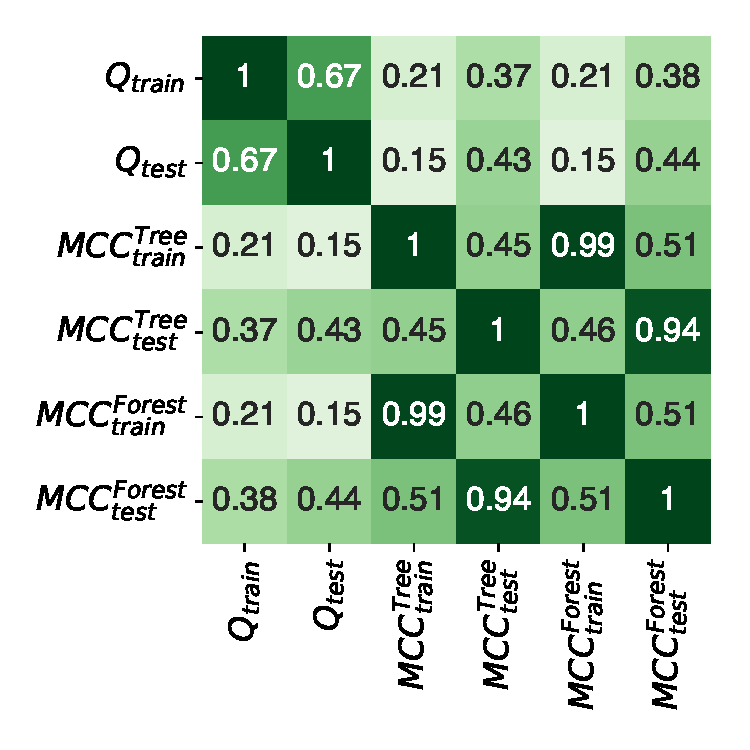
\includegraphics[width=0.7\textwidth]{plots/evaluation-metrics-correlation.pdf}
	\caption{Correlation between evaluation metrics over all experimental settings.}
	\label{fig:evaluation-metrics-correlation}
\end{figure}

As one can expect, the average prediction performance of random forests is higher than that of decision trees.
Also, overfitting occurs for both models, i.e., there is a gap between training-set and test-set prediction performance.
As we do not limit the growth of trees or prune them after training, this observation is expected.
However, that will not prevent our analysis how prediction performance develops over alternative feature sets, where we normalize feature-sets quality.
To a lesser extent, the optimization objective $Q$ also shows overfitting for all feature-selection methods.

Figure~\ref{fig:evaluation-metrics-correlation} shows the Spearman correlation between different evaluation metrics.
As the performance of decision trees and random forests is highly correlated on training set as well as test set, we only focus on one prediction model in the following:
We choose decision trees, as they always consider all features during training, while random forests involve random sampling of features.

Figure~\ref{fig:evaluation-metrics-correlation} also shows that the correlation between training-set quality and test-set quality is moderate, but not high, for the optimization objective $Q$ as well as prediction performance in terms of MCC.
This might be caused by different degrees of overfitting, depending on the experimental settings.
Further, the correlation between optimization objective $Q$ and prediction MCC is only weak to moderate.
This means that the quality criterion of feature selection is only partially indicative of prediction performance.
In particular, only one of our four feature-selection methods uses prediction performance to assess feature sets.

\subsection{Feature-Selection Methods}

As the different feature-selection methods have different functions as optimization objectives $Q$, it does not make sense to compare objective values between feature-selection methods.
Regarding the optimization status, we note that 89\% of feature sets for \emph{FCBF} could not be determined, as the solver timed out or the optimization problem was infeasible.
For MI, this figure only is 19\%.
Thus, besides the constraints for alternatives, the constraints in our formulation of \emph{FCBF} (c.f.~Equation~\ref{eq:fcbf}) made it hard to find valid feature sets.
This point needs to be considered when applying our \emph{FCBF} feature selector.

Regarding test-set prediction performance, \emph{Model Gain} beats \emph{MI} and \emph{Greedy Wrapper} on average.
The median test-set MCC for decision trees is 0.57 for \emph{Model Gain}, 0.54 for \emph{MI}, and 0.51 for \emph{Greedy Wrapper}.
It is not surprising that model-based importance yields better feature sets than univariate, model-free feature scoring with \emph{MI}.
The relatively bad performance of \emph{Greedy Wrapper} might result from its heuristic nature:
The wrapper search can only evaluate a fraction of all feasible feature sets and might get stuck in local optima, while the remaining feature-selection methods optimize globally.

The feature-set size $k$ shows the expected effect:
Larger feature sets, i.e., $k=10$, exhibit higher feature-set quality than smaller feature sets, i.e., $k=5$.
However, doubling the number of features does not double the prediction performance.
Over all experimental settings, the median test-set MCC for decision trees is 0.50 for $k=5$ and 0.60 for $k=10$.
This displays that small feature sets can already achieve a large share of the possible prediction performance.
For the optimization objective $Q$, the increase from $k=5$ to $k=10$ is higher than for prediction performance, but still less than proportional with $k$.

\subsection{Searching Alternatives}

\subsubsection{Search Method}

\begin{figure}[htb]
	\centering
	\begin{subfigure}{0.48\textwidth}
		\centering
		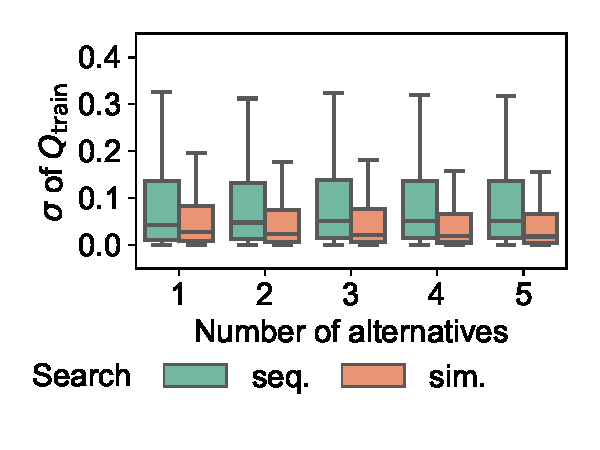
\includegraphics[width=\textwidth]{plots/impact-search-stddev-objective.pdf}
		\caption{Standard deviation of objective.}
		\label{fig:impact-search-stddev-objective}
	\end{subfigure}
	\hfill
	\begin{subfigure}{0.48\textwidth}
		\centering
		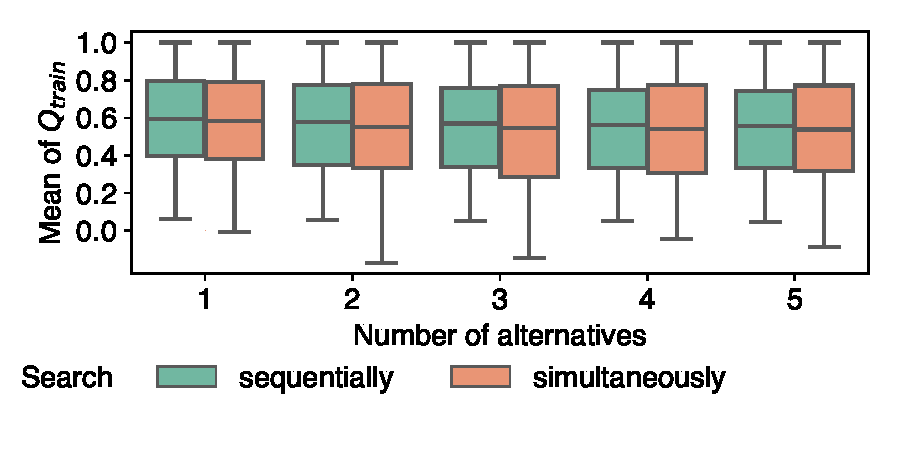
\includegraphics[width=\textwidth]{plots/impact-search-mean-objective.pdf}
		\caption{Mean objective.}
		\label{fig:impact-search-mean-objective}
	\end{subfigure}
	\caption{Training-set objective value $Q$ in experimental runs of sequential or simultaneous search.
	Outliers removed for readability reasons.}
	\label{fig:impact-search-objective}
\end{figure}

As we expected, the training-set objective value $Q$ of feature sets within a particular search run varies more for sequential search than for simultaneous search.
Figure~\ref{fig:impact-search-stddev-objective} visualizes this observation.
Also, this variation increases with the number of alternatives for sequential search, but decreases for simultaneous search.
I.e., simultaneous search finds relatively homogeneous feature sets, in particular, if many alternatives are desired.
On the test set, the objective value $Q$ of simultaneous-search feature sets still varies less than for sequential search, but increases with the number of alternatives.
This effect might be a result of overfitting.
Regarding test-set prediction performance, simultaneous search does not show lower variance than sequential search any more.

Surprisingly, the average feature-set quality of simultaneous search is not higher than for sequential search, neither regarding objective value $Q$ nor regarding prediction performance.
Figure~\ref{fig:impact-search-mean-objective} shows this behavior for the mean training-set objective of search runs.
Depending on the concrete search setting, either of the two search types might yield better-performing feature sets.
An explanation for this phenomenon is that search does not always yield the exact optimum.
For \emph{Greedy Wrapper}, the search is heuristic per se.
Additionally, the exact optimization of the other three feature-selection methods can time out.
As simultaneous search is harder than sequential search, it is affected stronger by this phenomenon.
In particular, 11.65\% of feature sets from simultaneous search might not be optimal, as the solver timed out.
This figure strongly depends on the number of alternatives:
While there are no or only a few such potentially sub-optimal feature sets for up to three alternatives in simultaneous search, 4\% of the feature sets might be suboptimal for four alternatives and 35\% of the feature sets for five alternatives.
For sequential search, we do not have any feasible but sub-optimal solution.

Based on these results, we focus on sequential search in the following.

\subsubsection{Number of Alternatives}

\begin{figure}[htb]
	\centering
	\begin{subfigure}{0.48\textwidth}
		\centering
		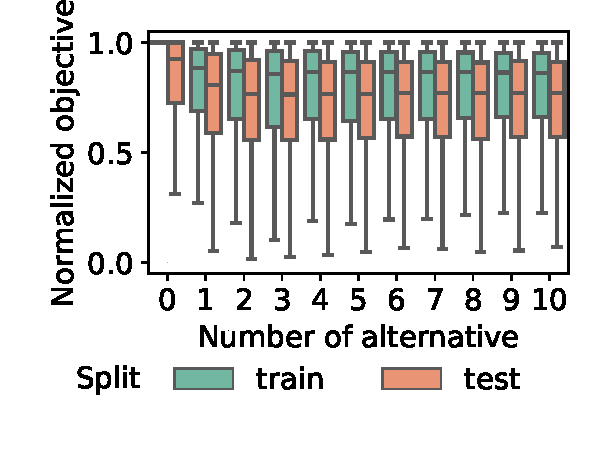
\includegraphics[width=\textwidth]{plots/impact-num-alternatives-objective-max.pdf}
		\caption{Max-normalization.}
		\label{fig:impact-num-alternatives-objective-max}
	\end{subfigure}
	\hfill
	\begin{subfigure}{0.48\textwidth}
		\centering
		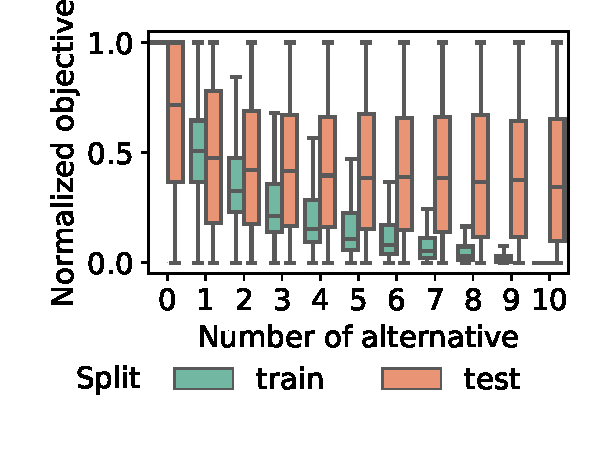
\includegraphics[width=\textwidth]{plots/impact-num-alternatives-objective-min-max.pdf}
		\caption{Min-max-normalization.}
		\label{fig:impact-num-alternatives-objective-min-max}
	\end{subfigure}
	\caption{Development of objective value $Q$, normalized per experimental setting, over the alternatives in sequential search, using \emph{MI} as feature selector.
	Outliers removed for readability reasons.}
	\label{fig:impact-num-alternatives-objective}
\end{figure}

For sequential search, the training-set objective value $Q$ naturally decreases with the number of alternatives, at least for the feature-selection criteria optimized exactly.
Figure~\ref{fig:impact-num-alternatives-objective} illustrates this for \emph{MI}-based feature selection.
The other feature-selection methods, including the heuristic \emph{Greedy Wrapper}, exhibit similar effects.
As feature-set quality varies between datasets and number of features $k$, we apply normalization:
In Figure~\ref{fig:impact-num-alternatives-objective-max}, we have max-normalized the objective value for each search of alternatives, i.e., one feature set from a search run gets an objective of 1 and the other feature-set qualities are scaled accordingly.
This figure shows that there might be multiple alternatives of similar quality, as the median feature-set quality remains relatively stable over the number of alternatives, and is close to the maximum of 1.
Figure~\ref{fig:impact-num-alternatives-objective-min-max} uses min-max normalization, i.e., the worst of the alternatives gets an objective of 0.
This figure highlights that the decrease training-set objective value is most prominent from the original feature set to the first alternative, but becomes smaller beyond.

Figure~\ref{fig:impact-num-alternatives-objective} also shows that test-set objective value drops the most from the original feature set to the first alternative as well.
The decrease in median objective value over the alternatives is less visible than on the training set.
In particular, alternatives can even have a higher objective value than the original feature set, due to overfitting of the optimization procedure.
Similar findings hold for test-set prediction performance.
Thus, the alternative feature sets fulfill their purpose of being different solutions with similar quality.

However, one should note that these observations refer to the quality of the feature sets actually found.
In particular, the more alternatives are desired, the more likely it is that the optimization problem becomes infeasible.
For example, the \emph{MI} feature selector in sequential search always returns a solution for the original feature set, but the problem is infeasible in 2\% of the cases for the first alternative, 14\% of the cases for the second alternative, 24\% of the cases for the fifth alternative, and 30\% of the cases for the tenth alternative.
Thus, while the quality of feature-sets remains relatively stable with increased number of alternatives, valid alternatives might simply not exist.
This outcome depends on the dissimilarity, threshold $\tau$, which we analyze in the following.

\subsubsection{Dissimilarity Threshold $\tau$}

\begin{figure}[htb]
	\centering
	\begin{subfigure}{0.48\textwidth}
		\centering
		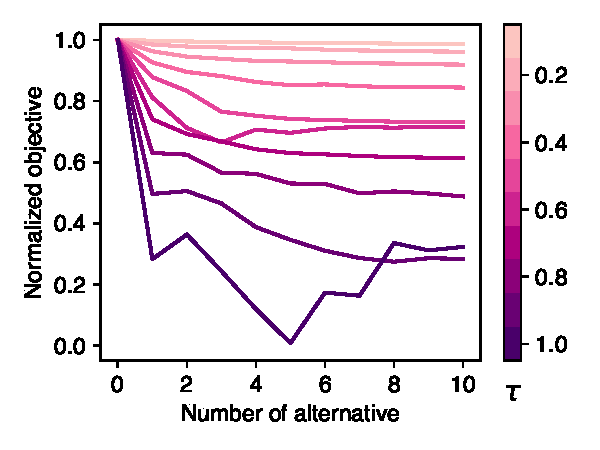
\includegraphics[width=\textwidth]{plots/impact-num-alternatives-train-objective-tau.pdf}
		\caption{Training set.}
		\label{fig:impact-num-alternatives-train-objective-tau}
	\end{subfigure}
	\hfill
	\begin{subfigure}{0.48\textwidth}
		\centering
		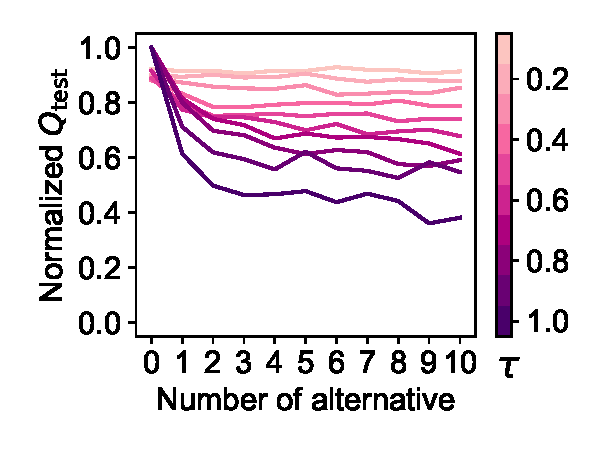
\includegraphics[width=\textwidth]{plots/impact-num-alternatives-test-objective-tau.pdf}
		\caption{Test set.}
		\label{fig:impact-num-alternatives-test-objective-tau}
	\end{subfigure}
	\caption{Development of median objective value $Q$, max-normalized per experimental setting, over the alternatives and dissimilarity threshold $\tau$ in sequential search, using \emph{MI} as feature selector and $k=10$.}
	\label{fig:impact-num-alternatives-objective-tau}
\end{figure}

As Figure~\ref{fig:impact-num-alternatives-objective-tau} shows for \emph{MI} as feature selector, the decrease of the objective value $Q$ over the number of alternatives can strongly depend on the dissimilarity threshold $\tau$.
If the dissimilarity requirement is low, e.g., $\tau=0.1$, the objective value barely drops over the number of alternatives.
In contrast, if the dissimilarity threshold is be high, e.g, $tau=1$, the objective decrease significantly.
This phenomenon also holds for test-set objective and test-set prediction performance, though the decrease with $\tau$ is less prominent for prediction performance.
Also, the the number of infeasible optimization problems increases with $tau$:
For a higher dissimilarity threshold, the likelihood is higher that there is no feature set that is alternative enough.

While the previous observation were made for \emph{MI} as feature selector, they do not hold universally.
Besides \emph{MI}, the results for \emph{Model Gain} strongly depend on \emph{tau} as well.
In contrast, \emph{FCBF} and \emph{Greedy Wrapper} exhibit less influence of $\tau$ on feature-set quality.
In case of \emph{Greedy Wrapper}, this can be explained by its heuristic search procedure.
In case of \emph{FCBF}, the fraction of infeasible solutions is much higher than for \emph{MI} in general, so adding further constraints has less impact.

\section{Conclusions and Future Work}
\label{sec:conclusion}

\subsection{Conclusions}

- alternatives are interesting
- existing fs methods not sufficient
- we are general regarding FS method and can also integrate other kinds of constraints
TODO: adapt abstract and intro to results

\subsection{Future Work}

- other FS techniques, in particular, embedded approaches
- other set-dissimilarity measures and other aggregations (than "all are alternative") for multi-alternative case
- soft constraints or multi-objective (Pareto) approach for problem (rather than hard constraints)

\printbibliography

\end{document}
